% Design note, CS4.406 Assignment 2. Build from this directory:
%   python make_tables.py && pdflatex design-note.tex && pdflatex design-note.tex
% Every table under tables/ and every number macro in tables/numbers.tex is generated from
% results/*.json by make_tables.py; none is typed by hand.
\documentclass[11pt,twocolumn]{article}

\usepackage[margin=1in]{geometry}
\usepackage[T1]{fontenc}
\usepackage{lmodern}
\usepackage{microtype}
\usepackage{booktabs}
\usepackage{tabularx}
\usepackage{array}
\usepackage{multirow}
\usepackage{graphicx}
\usepackage{float}
\usepackage{xcolor}
\usepackage[shortlabels]{enumitem}
\usepackage[font=small,labelfont=bf,skip=4pt]{caption}
\usepackage{titlesec}
\usepackage{tikz}
\usetikzlibrary{arrows.meta,positioning,fit,calc}
\usepackage{pgfplots}
\pgfplotsset{compat=1.17}
\usepackage[colorlinks=true,linkcolor=black,citecolor=black,urlcolor=blue!50!black]{hyperref}

% Two-column at 11pt gives a 3.4in measure. Without a wider gutter and tolerant line
% breaking, dense text full of inline code overflows constantly.
\setlength{\columnsep}{20pt}
\tolerance=1500
\emergencystretch=2em
\hbadness=4000
\setlist{nosep,leftmargin=*}
\titlespacing*{\section}{0pt}{9pt}{4pt}
\titlespacing*{\subsection}{0pt}{6pt}{2pt}
\setlength{\parskip}{3pt}
\setlength{\parindent}{0pt}
\setlength{\textfloatsep}{8pt plus 2pt minus 2pt}
\setlength{\floatsep}{8pt plus 2pt minus 2pt}
\renewcommand{\arraystretch}{1.08}
\renewcommand{\topfraction}{0.85}
\renewcommand{\bottomfraction}{0.7}
\renewcommand{\textfraction}{0.12}
\renewcommand{\floatpagefraction}{0.75}

% Short forms used throughout.
\newcommand{\eb}{EB-NeRD}
\newcommand{\mind}{MIND}
\newcommand{\feat}[1]{\texttt{\detokenize{#1}}}
\newcommand{\pend}[1]{\textcolor{red!70!black}{\textbf{[#1]}}}
% A term being defined for the first time.
\newcommand{\term}[1]{\textit{#1}}
% A metric cell: mean on the first line, its 95% interval beneath in small type.
\newcommand{\cellci}[3]{\begin{tabular}[t]{@{}c@{}}#1\\[-2pt]{\scriptsize[#2, #3]}\end{tabular}}
\newcommand{\cellcib}[3]{\begin{tabular}[t]{@{}c@{}}\textbf{#1}\\[-2pt]{\scriptsize[#2, #3]}\end{tabular}}
% A difference cell: the signed delta, with its already-formatted interval beneath.
\newcommand{\dcell}[2]{\begin{tabular}[t]{@{}c@{}}#1\\[-2pt]{\scriptsize #2}\end{tabular}}

\IfFileExists{tables/numbers.tex}{\newcommand{\BenchAnnGrowth}{26.8}
\newcommand{\BenchAnnPninetynine}{48.1}
\newcommand{\BenchAnnShare}{44}
\newcommand{\BenchBmGrowth}{16.2}
\newcommand{\BenchCapacityQPS}{188}
\newcommand{\BenchCores}{8}
\newcommand{\BenchCorpusGrowth}{10.0}
\newcommand{\BenchCost}{0.000472}
\newcommand{\BenchFaissFull}{60.8}
\newcommand{\BenchFaissSmall}{6.1}
\newcommand{\BenchFeatGrowth}{2.9}
\newcommand{\BenchFeatures}{22}
\newcommand{\BenchHeadroom}{1.3}
\newcommand{\BenchPfifty}{42.5}
\newcommand{\BenchPninetyfive}{64.7}
\newcommand{\BenchPninetynine}{77.3}
\newcommand{\BenchRequests}{2,000}
\newcommand{\BenchRerankGrowth}{7.6}
\newcommand{\BenchRerankPninetynine}{34.7}
\newcommand{\BenchRerankShare}{39}
\newcommand{\BenchSerialQPS}{24}
\newcommand{\BenchTokGrowth}{4.6}
\newcommand{\BenchTrees}{399}
\newcommand{\EBColdThrTest}{34}
\newcommand{\EBColdThrVal}{42}
\newcommand{\EBFinalTest}{0.7908}
\newcommand{\EBFinalVal}{0.7885}
\newcommand{\EBFusedTest}{0.5380}
\newcommand{\EBFusedVal}{0.5528}
\newcommand{\EBGainTest}{$+$0.2528}
\newcommand{\EBGainTestCI}{[$+$0.2514, $+$0.2543]}
\newcommand{\EBGainVal}{$+$0.2357}
\newcommand{\EBGainValCI}{[$+$0.2329, $+$0.2385]}
\newcommand{\EBHeadThrTest}{349}
\newcommand{\EBHeadThrVal}{379}
\newcommand{\EBLeakyTest}{0.5797}
\newcommand{\EBLeakyVal}{0.5784}
\newcommand{\HistFull}{29.1}
\newcommand{\HistSmall}{3.6}
\newcommand{\LadderExpMindTest}{$+$0.0297}
\newcommand{\LadderExpMindTestCI}{[$+$0.0278, $+$0.0316]}
\newcommand{\LadderExpMindTestFrom}{0.6666}
\newcommand{\LadderExpMindTestTo}{0.6964}
\newcommand{\LadderExpMindVal}{$+$0.0458}
\newcommand{\LadderExpMindValCI}{[$+$0.0440, $+$0.0478]}
\newcommand{\LadderExpMindValFrom}{0.6539}
\newcommand{\LadderExpMindValTo}{0.6997}
\newcommand{\LadderExpTest}{$+$0.0255}
\newcommand{\LadderExpTestCI}{[$+$0.0249, $+$0.0261]}
\newcommand{\LadderExpTestFrom}{0.7653}
\newcommand{\LadderExpTestTo}{0.7908}
\newcommand{\LadderExpVal}{$+$0.0249}
\newcommand{\LadderExpValCI}{[$+$0.0238, $+$0.0261]}
\newcommand{\LadderExpValFrom}{0.7636}
\newcommand{\LadderExpValTo}{0.7885}
\newcommand{\LadderSevenTest}{$+$0.0130}
\newcommand{\LadderSevenTestCI}{[$+$0.0124, $+$0.0134]}
\newcommand{\LadderSevenTestFrom}{0.7523}
\newcommand{\LadderSevenTestTo}{0.7653}
\newcommand{\LadderSevenVal}{$+$0.0113}
\newcommand{\LadderSevenValCI}{[$+$0.0104, $+$0.0122]}
\newcommand{\LadderSevenValFrom}{0.7523}
\newcommand{\LadderSevenValTo}{0.7636}
\newcommand{\MDColdThrTest}{3}
\newcommand{\MDColdThrVal}{4}
\newcommand{\MDFinalTest}{0.6964}
\newcommand{\MDFinalVal}{0.6997}
\newcommand{\MDFusedTest}{0.6381}
\newcommand{\MDFusedVal}{0.6390}
\newcommand{\MDGainTest}{$+$0.0583}
\newcommand{\MDGainTestCI}{[$+$0.0565, $+$0.0603]}
\newcommand{\MDGainVal}{$+$0.0607}
\newcommand{\MDGainValCI}{[$+$0.0587, $+$0.0628]}
\newcommand{\MDHeadThrTest}{152}
\newcommand{\MDHeadThrVal}{205}
\newcommand{\PoolFull}{388}
\newcommand{\PoolGrowth}{1.13}
\newcommand{\PoolSmall}{345}
\newcommand{\QnineCI}{[$+$0.0212, $+$0.0240]}
\newcommand{\QnineCausal}{0.7523}
\newcommand{\QnineDelta}{$+$0.0226}
\newcommand{\QnineLeaky}{0.7749}
\newcommand{\TokFull}{144.6}
\newcommand{\TokGrowth}{8.2}
\newcommand{\TokSmall}{17.7}
}{}

\title{\vspace{-2.4em}{\Large\textbf{Learning from Click-Logs: a Two-Stage News Recommender
for \eb{} and \mind{}}}\\[5pt]
\normalsize Design note, CS4.406 Information Retrieval \& Extraction, Assignment 2}
\author{Naman Singhal (2024114013) \qquad Yash More (2024114004)}
\date{}

\begin{document}
\maketitle
\vspace{-2em}

\section*{Summary}

A two-stage news recommender for \eb{}~\cite{kruse2024} and \mind{}~\cite{wu2020mind}: cheap
retrieval narrows the catalogue to 200 candidates, then a LightGBM LambdaRank model re-ranks them
on 22 click-log features, all restricted to data from strictly before the impression predicted.

\begin{itemize}
\item The behavioural axis is what matters. On \eb{} the re-ranker scores \EBFinalTest{}
  test AUC against \EBFusedTest{} for retrieval alone, a gain of \EBGainTest{} \EBGainTestCI.
  Popularity carries most of it: a model given popularity and nothing else already reaches 0.7348.
  Because that signal needs no history, cold-start and warm users gain equally (0.7910 and 0.7908),
  but the re-ranker is \emph{worse} than retrieval on the most popular articles.
\item The same architecture is worth far less on \mind{}, \MDGainTest{} \MDGainTestCI{}
  test, because five of the 22 features have no source there: a measured property of the data, not
  a failure to reproduce.
\item We reproduced NRMS and beat it with one change, a longer user history:
  $+$0.0094 [$+$0.0086, $+$0.0102] test AUC. Our re-ranker sits about 0.19 AUC above it, because
  NRMS never sees the click log's popularity signal.
\item Honesty is nearly free. Serving-unavailable features would add only \QnineDelta{}
  \QnineCI, against the \EBGainTest{} the behavioural axis earns legitimately. We found and fixed a
  future-click leak contaminating 99.8\% of validation impressions; fixing it \emph{raised} test
  accuracy.
\item Serving fits the budget, and exact search breaks at scale. A single request takes
  \BenchPfifty{} ms at the median and \BenchPninetynine{} ms at p99, inside a 100 ms target. At
  10$\times$ the catalogue exact embedding search grows \BenchAnnGrowth$\times$ and becomes the
  bottleneck; the candidate pool stays flat at \PoolGrowth$\times$, so the other stages do the same
  work more slowly.
\item What we upload is not what we report, and we say so: Codabench withholds the click
  labels, so the submitted model drops five popularity features and scores 0.7351 against
  \EBFinalTest{} on our own test split.
\end{itemize}

\section{What we built}
\label{sec:system}

The task is news recommendation from click-logs. The unit of everything is an \term{impression}:
at time $t$ a user is shown a list of \term{candidate} articles and clicks some of them. Our job is
to order each impression's candidates so the clicked ones come first. We extend our two
Assignment-1 retrieval systems (lexical and semantic) with the \term{behavioural} signal in the
logs: what users clicked, how often each article has been clicked or shown, and how fresh it is.

\subsection{Data and evaluation protocol}

\begin{table*}[t]
\centering\footnotesize
\begin{tabular}{@{}lrcrr@{}}
\toprule
 & & & \multicolumn{2}{c}{leaderboard test set} \\
\cmidrule(l){4-5}
dataset & articles & train / val / test impressions & impressions & articles \\
\midrule
\eb{} small (Danish) & 20,738 & 168,522 / 64,365 / 244,647 & 13,536,710 & 125,500 \\
\mind{} small (English) & 65,238 & 95,071 / 61,894 / 73,152 & 2,370,727 & 120,961 \\
\bottomrule
\end{tabular}
\caption{Development data and the held-out leaderboard sets. Splits are temporal: every train
impression precedes every val impression, which precedes every test impression.}
\label{tab:data}
\end{table*}

\textbf{Splits are by time, never random.} A random split would let the model learn from
Thursday to predict Wednesday, which no deployed system can do. \eb{} val begins 23 May 07:00 and
test 25 May 07:00; \mind{} uses the last day of its training log as val and its dev log as test.

\textbf{Metric: per-impression AUC}, computed inside each impression and averaged over those with
both a click and a non-click. We never pool candidates across impressions, because the ranking is
only judged inside one: pooling rewards features that merely differ between impressions, and the
effect is large, with article freshness reading 0.5861 pooled against 0.5087 per impression.

\textbf{Significance: paired bootstrap 95\% intervals} \cite{efron1993}, 1,000 resamples, both
systems scored on the \emph{same} resampled impressions so their correlated errors cancel. A gain
counts only if its interval excludes zero. Selection happens on val; test is scored once.

\subsection{Architecture: retrieve, then re-rank}

\begin{figure*}[t]
\centering
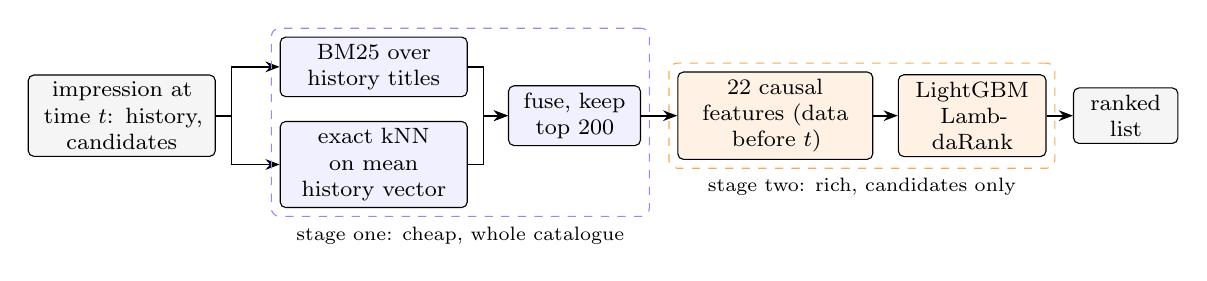
\begin{tikzpicture}[
  box/.style={draw, rounded corners=2pt, align=center, font=\footnotesize, inner sep=2.5pt,
              minimum height=7mm, text width=#1},
  arr/.style={-{Stealth[length=1.8mm]}, semithick}]
\node[box=2.2cm, fill=gray!8] (imp) at (0,0) {impression at time $t$: history, candidates};
\node[box=2.2cm, fill=blue!6] (bm25) at (3.2,0.62) {BM25 over history titles};
\node[box=2.2cm, fill=blue!6] (ann) at (3.2,-0.62) {exact kNN on mean history vector};
\node[box=1.5cm, fill=blue!6] (fuse) at (5.75,0) {fuse, keep top 200};
\node[box=2.3cm, fill=orange!10] (feat) at (8.3,0) {22 causal features (data before $t$)};
\node[box=1.7cm, fill=orange!10] (lgb) at (10.8,0) {LightGBM LambdaRank};
\node[box=1.15cm, fill=gray!8] (out) at (12.75,0) {ranked list};
\draw[arr] (imp.east) -- ++(0.2,0) |- (bm25.west);
\draw[arr] (imp.east) -- ++(0.2,0) |- (ann.west);
\draw[arr] (bm25.east) -- ++(0.2,0) |- (fuse.west);
\draw[arr] (ann.east) -- ++(0.2,0) |- (fuse.west);
\draw[arr] (fuse) -- (feat);
\draw[arr] (feat) -- (lgb);
\draw[arr] (lgb) -- (out);
\node[draw=blue!45, dashed, rounded corners=3pt, fit=(bm25)(ann)(fuse), inner sep=3pt,
      label={[font=\scriptsize]below:stage one: cheap, whole catalogue}] {};
\node[draw=orange!70, dashed, rounded corners=3pt, fit=(feat)(lgb), inner sep=3pt,
      label={[font=\scriptsize]below:stage two: rich, candidates only}] {};
\end{tikzpicture}
\caption{The two-stage pipeline. Stage one touches every article, so it must stay cheap per
article. Stage two touches only the candidates, so it can afford per-candidate features.}
\label{fig:pipeline}
\end{figure*}

\textbf{Stage one, candidate generation} (carried from Assignment 1). \emph{BM25}
\cite{robertson2009,lu2024bm25s} is a lexical score: the query is the titles of the user's last
$N$ clicks ($N=30$ on \eb{}, $100$ on \mind{}), and an article scores highly when it shares rare
words with them. Stemming is on for both languages and a Danish stopword list is applied. The
\emph{semantic} retriever represents the user as the mean of their clicked articles' vectors and
finds the nearest articles by cosine with an exact FAISS \texttt{IndexFlatIP} \cite{johnson2019faiss}.
Vectors are the provided 768-dimensional \texttt{contrastive\_vector} for \eb{} and
384-dimensional \texttt{all-MiniLM-L6-v2} \cite{reimers2019} for \mind{}, both chosen by measurement
in Assignment 1. The two scores are standardised within each candidate pool and mixed linearly,
with the weight chosen on val. Each retriever keeps its top 200 candidates. Both indexes are held
in RAM.

\textbf{Stage two, the re-ranker.} A LightGBM \cite{ke2017lightgbm} gradient-boosted tree model
with the \term{LambdaRank} objective \cite{burges2010}. LambdaRank learns from pairs of candidates
inside the same impression and weights each pair by how much swapping them would change nDCG, so
training optimises the ranking itself rather than a click probability. We measured this choice
rather than assuming it (Table~\ref{tab:choices}). Settings: learning rate 0.05, 31 leaves,
at least 50 rows per leaf, 90\% feature and row subsampling, up to 400 rounds with early stopping
on val nDCG, seed 13.

\subsection{Features and the behaviour-window boundary}

\textbf{Every feature for an impression at time $t$ uses only data from strictly before $t$.} We
call this the \term{behaviour-window boundary}. Click and exposure counts are computed by binary
search over each article's sorted event times with a strict ``$< t$'' cut, so an event at exactly
$t$ is excluded. Tests assert the boundary on every split, and each test was checked by injecting a
future click and confirming it fails (Section~\ref{sec:q9}).

\begin{table*}[t]
\centering\small
\begin{tabularx}{\linewidth}{@{}l>{\raggedright\arraybackslash}Xcc@{}}
\toprule
family & features and what they measure & \eb{} & \mind{} \\
\midrule
stage-one scores & \feat{bm25}, \feat{emb} (the two retrieval scores); \feat{emb_rank} (the
embedding score's rank inside the impression) & yes & yes \\
click popularity & \feat{pop_causal}: clicks before $t$ in a 6\,h window (unbounded on \mind{});
\feat{pop_24h}: the same over 24\,h; \feat{pop_velocity}: their ratio, ``rising now'' versus
``steadily popular''; \feat{pop_rank}, \feat{pop_rel_max}: standing among this impression's
candidates & yes & yes \\
exposure & the same five shapes (\feat{exp_causal}, \feat{exp_24h}, \feat{exp_velocity},
\feat{exp_rank}, \feat{exp_rel_max}) counting how often an article was \emph{shown} before $t$ &
yes & yes \\
user match & \feat{cat_match}: share of the user's history in the candidate's category;
\feat{ent_overlap}: shared named entities with the history & yes & yes \\
context & \feat{hist_len}: history length; \feat{n_cands}: number of candidates in the impression &
yes & yes \\
freshness & \feat{age_hours}, \feat{recency} (24\,h half-life decay of age) & yes & no \\
engagement & \feat{user_read}, \feat{user_scroll}: mean read time and scroll depth of past clicks;
\feat{engage_sim}: cosine to a read-time-weighted user vector & yes & no \\
\midrule
total & & 22 & 17 \\
\bottomrule
\end{tabularx}
\caption{The re-ranker's features. Rank and relative features exist because the metric is decided
inside one impression: a popularity of 200 dominates a quiet impression and is ordinary in a busy
one.}
\label{tab:features}
\end{table*}

\textbf{Five features cannot exist on \mind{}, and we drop them explicitly.} \mind{}'s publication
time is null for all 65,238 articles, and it ships no read-time or scroll data at all. A column of
zeros looks like a real feature to LightGBM, so the builder refuses to emit any feature that is
all-null or constant. This matches the data audit we did before designing features: \eb{} is rich
in behavioural signal, \mind{} has little beyond the click itself.

\textbf{Exposure} (``how often was this article shown before $t$'') was added for a practical
reason and kept for a better one. The leaderboard test files withhold the clicks, so click
popularity cannot be computed there (Section~\ref{sec:leaderboard}), but the lists of shown
articles are present. A live recommender also knows its own exposure log immediately, while click
feedback arrives later, so exposure is arguably the more realistic signal.

\section{Results}
\label{sec:results}

Unless stated otherwise, numbers are per-impression AUC on \eb{} small and \mind{} small, with
paired bootstrap 95\% intervals, selected on val and scored once on test.

\subsection{Before and after re-ranking}
\label{sec:beforeafter}

\begin{table*}[t]
\centering\scriptsize
\begin{tabular}{@{}lccccc@{}}
\toprule
system & AUC & MRR & MRR, all clicks & nDCG@5 & nDCG@10 \\
\midrule
\multicolumn{6}{@{}l}{\textit{\eb{} small, test}} \\
BM25 (stage one) & \cellci{0.5107}{0.5094}{0.5120} & \cellci{0.3257}{0.3245}{0.3269} & \cellci{0.3253}{0.3241}{0.3264} & \cellci{0.3577}{0.3563}{0.3591} & \cellci{0.4409}{0.4397}{0.4420} \\[2pt]
embeddings (stage one) & \cellci{0.5397}{0.5384}{0.5409} & \cellci{0.3492}{0.3480}{0.3503} & \cellci{0.3487}{0.3475}{0.3498} & \cellci{0.3831}{0.3818}{0.3845} & \cellci{0.4627}{0.4616}{0.4638} \\[2pt]
fused (stage one) & \cellci{0.5380}{0.5367}{0.5392} & \cellci{0.3474}{0.3463}{0.3486} & \cellci{0.3470}{0.3458}{0.3481} & \cellci{0.3813}{0.3800}{0.3827} & \cellci{0.4613}{0.4602}{0.4624} \\[2pt]
two-stage re-ranker & \cellcib{0.7908}{0.7898}{0.7918} & \cellcib{0.5685}{0.5671}{0.5699} & \cellcib{0.5678}{0.5665}{0.5693} & \cellcib{0.6330}{0.6318}{0.6344} & \cellcib{0.6650}{0.6639}{0.6662} \\[2pt]
fused + lifetime popularity$^\ast$ & \cellci{0.5797}{0.5785}{0.5810} & \cellci{0.3688}{0.3677}{0.3700} & \cellci{0.3684}{0.3672}{0.3696} & \cellci{0.4101}{0.4088}{0.4115} & \cellci{0.4841}{0.4830}{0.4852} \\[2pt]
\midrule
\multicolumn{6}{@{}l}{\textit{\mind{} small, test}} \\
BM25 (stage one) & \cellci{0.5685}{0.5663}{0.5706} & \cellci{0.3108}{0.3085}{0.3133} & \cellci{0.2693}{0.2673}{0.2717} & \cellci{0.2868}{0.2844}{0.2894} & \cellci{0.3479}{0.3456}{0.3504} \\[2pt]
embeddings (stage one) & \cellci{0.6369}{0.6347}{0.6390} & \cellci{0.3510}{0.3486}{0.3535} & \cellci{0.3061}{0.3039}{0.3085} & \cellci{0.3341}{0.3316}{0.3367} & \cellci{0.3937}{0.3913}{0.3961} \\[2pt]
fused (stage one) & \cellci{0.6381}{0.6358}{0.6402} & \cellci{0.3536}{0.3511}{0.3561} & \cellci{0.3075}{0.3053}{0.3098} & \cellci{0.3361}{0.3335}{0.3388} & \cellci{0.3956}{0.3934}{0.3981} \\[2pt]
two-stage re-ranker & \cellcib{0.6964}{0.6943}{0.6983} & \cellcib{0.4027}{0.4001}{0.4054} & \cellcib{0.3459}{0.3436}{0.3483} & \cellcib{0.3854}{0.3827}{0.3882} & \cellcib{0.4458}{0.4435}{0.4483} \\[2pt]
\bottomrule
\end{tabular}

\caption{All accuracy metrics on the test split, with 95\% bootstrap intervals beneath each mean.
``Stage one'' rows are the retrieval scores ranking the same candidates; the re-ranker reorders
them. $^\ast$Lifetime popularity is not available at serving time and is reported only to price
what it would buy (Section~\ref{sec:q9}). Validation-split figures are in Appendix~\ref{app:val}.}
\label{tab:overall}
\end{table*}

\textbf{Two baselines appear in this report and they are not the same thing.} Here ``stage one''
is the fused retrieval score ranking the candidates directly (\EBFusedTest{} on test). The
ablation grid in Table~\ref{tab:choices} instead compares against \feat{stage1_only}, a ranker
trained on the two retrieval scores alone, which is slightly stronger at 0.5430. That is why the
same result reads \EBGainTest{} here and $+$0.2223 there.

\textbf{On \eb{} the re-ranker is worth \EBGainTest{} AUC} over fused retrieval,
\EBGainTestCI{} on test, and \EBGainVal{} \EBGainValCI{} on val. The val and test intervals
overlap, so the gain generalises across the time boundary rather than being an artefact of what we
selected on. Every other accuracy metric moves the same way, so this is a genuine reordering rather
than a trade between metrics.

\textbf{On \mind{} the same architecture is worth \MDGainTest{} \MDGainTestCI{}}, far less. Two
things compound. Five of the 22 features have no source in \mind{}, including every freshness and
engagement signal, so the behavioural axis is thinner. And \mind{}'s stage one is already stronger
in absolute terms (\MDFusedTest{} against \eb{}'s \EBFusedTest{}), which leaves less headroom to
begin with. We report the contrast rather than presenting one system that is quietly two: a
smaller gain on a dataset with less signal is a measured property of the data.

\textbf{One family of features did transfer, and it was the one built under duress.} An earlier
round of seven features moved \mind{} by nothing significant at all. The five exposure features,
added because Codabench withholds the click labels, are worth \LadderExpMindTest{}
\LadderExpMindTestCI{} on \mind{} test and \LadderExpMindVal{} \LadderExpMindValCI{} on val. How
often an article was \emph{shown} is apparently a signal both corpora carry, where freshness and
engagement are specific to \eb{}.

\subsection{What each design choice was worth}
\label{sec:choices}

Every choice below was made by measuring the alternative, one change at a time, with a paired
bootstrap interval. Rows marked ``10 features'' were measured before the feature set grew; the two
feature rows are the incremental steps to the shipped \eb{} model.

\begin{table*}[t]
\centering\footnotesize
\begin{tabularx}{\linewidth}{@{}>{\raggedright\arraybackslash}X>{\raggedright\arraybackslash}p{2.35cm}cc>{\raggedright\arraybackslash}p{1.75cm}@{}}
\toprule
choice & compared against & val $\Delta$ [95\% CI] & test $\Delta$ [95\% CI] & verdict \\
\midrule
re-ranking at all & stage one alone & \dcell{$+$0.2138}{[$+$0.2110, $+$0.2168]} & \dcell{$+$0.2223}{[$+$0.2209, $+$0.2238]} & core result \\
LambdaRank objective (10 features) & binary objective & \dcell{$+$0.0161}{[$+$0.0150, $+$0.0173]} & \dcell{$+$0.0165}{[$+$0.0159, $+$0.0171]} & kept \\
6\,h click-popularity window (10 features) & all past clicks & \dcell{$+$0.0034}{[$+$0.0026, $+$0.0043]} & \dcell{$+$0.0062}{[$+$0.0058, $+$0.0067]} & shipped \\
seven rank, velocity and context features & the 10 features & \dcell{\LadderSevenVal}{\LadderSevenValCI} & \dcell{\LadderSevenTest}{\LadderSevenTestCI} & shipped \\
five exposure features & the 17 features & \dcell{\LadderExpVal}{\LadderExpValCI} & \dcell{\LadderExpTest}{\LadderExpTestCI} & shipped \\
read-time-weighted user vector & uniform vector only & \dcell{$+$0.0003}{[$-$0.0003, $+$0.0010]} & \dcell{$+$0.0005}{[$+$0.0002, $+$0.0008]} & kept, tiny \\
linear fusion of BM25 and embeddings & embeddings alone & \dcell{$+$0.0022}{[$+$0.0010, $+$0.0034]} & \dcell{$-$0.0017}{[$-$0.0023, $-$0.0010]} & does not generalise \\
title-only BM25 documents & title and abstract & \dcell{$+$0.0025}{[$+$0.0002, $+$0.0047]} & \dcell{$+$0.0043}{[$+$0.0031, $+$0.0055]} & not shipped$^\dagger$ \\
stemming off, \mind{} & stemming on & \dcell{$-$0.0023}{[$-$0.0034, $-$0.0013]} & \dcell{$-$0.0028}{[$-$0.0039, $-$0.0018]} & keep on \\
stemming off, \eb{} & stemming on & \dcell{$-$0.0003}{[$-$0.0019, $+$0.0014]} & \dcell{$-$0.0002}{[$-$0.0011, $+$0.0007]} & keep on, for cost \\
\bottomrule
\end{tabularx}
\caption{Per-impression AUC change from each choice, on \eb{} unless marked. The first row is the
\feat{stage1_only} arm of the 17-feature grid. $^\dagger$Title-only documents also cost val
recall@200 by $-$0.0024 [$-$0.0035, $-$0.0013], and recall is what stage two consumes.}
\label{tab:choices}
\end{table*}

Three rows deserve a sentence. The objective matters because a binary one leans on absolute
freshness, while LambdaRank leans on popularity contrasts inside the impression, which is what
decides the ranking. Counting only the last 6 hours of clicks asks how popular an article is right
now rather than how popular it has ever been; in isolation that moved the feature from 0.6902 to
0.7349, though inside the ranker the gain is far smaller because other features cover for it, so we
quote the ranker figure. Fusion is the awkward one: it helps on val and hurts on test, both
significantly, so the mixing weight does not transfer across the time boundary. That is moot next
to stage two, but it is an honest negative result.

\subsection{Baseline reproduced, then beaten (\eb{})}
\label{sec:baseline}

\textbf{The baseline.} NRMS \cite{wu2019nrms} is a neural recommender with two parts: a news
encoder that turns each article into a vector, and a user encoder that uses attention over the
user's clicked articles to decide which past clicks matter for the current prediction. We ran the
organisers' \texttt{ebnerd\_nrms\_docvec.py} unmodified on \eb{} small with the provided document
vectors, history size 20, 4 negatives per positive, batch 32 and seed 16. It reached val AUC
\textbf{0.6484} (best epoch 3, early-stopped at 7, 54 minutes on 16 CPU cores of a cluster node).

\textbf{That number is not comparable to ours.} The benchmark script trains on the organisers'
train and validation blocks together and validates on its own last day, which in our split means
it trains on our val and test impressions. So we also drove the same model, settings, vectors and
data loader from our temporal split: train on our train, stop early on our val, score our test
once. That run is the baseline we compare against.

\begin{table}[tb]
\centering\small
\begin{tabular}{@{}lcc@{}}
\toprule
\eb{} small, our temporal split & val AUC & test AUC \\
\midrule
NRMS, benchmark script and protocol (not comparable) & 0.6484 & -- \\
NRMS baseline, history size 20 & 0.5969 & 0.5938 \\
NRMS improved, history size 50 & 0.6042 & 0.6032 \\
\quad improved $-$ baseline & \dcell{$+$0.0072}{[$+$0.0058, $+$0.0088]} & \dcell{$+$0.0094}{[$+$0.0086, $+$0.0102]} \\
\midrule
our two-stage re-ranker & \EBFinalVal & \EBFinalTest \\
\bottomrule
\end{tabular}
\caption{NRMS reproduced and beaten with one change, paired bootstrap. Both NRMS arms score the
identical 64,365 val and 244,647 test impressions, aligned by impression id.}
\label{tab:nrms}
\end{table}

\textbf{The one principled change: a longer history, 20 to 50 clicks.} The motivation is our own
measurement. On clean data, the mean-of-history user vector improves steadily as the history
grows, from 0.5416 at 10 clicks to 0.5545 at 100 (Appendix~\ref{app:sweeps}). NRMS builds its user
representation from exactly that history, so it should benefit too. It does: the gain is
significant on both splits and larger on test than on val, the opposite of what over-fitting to
val would produce. We stopped at 50 because attention cost grows with the square of the history
length. A guard asserts every article id reaches the model (coverage 1.0000 on all four checks),
since a silent id mismatch would train on zero vectors and still report a believable AUC.

\textbf{Why our system beats NRMS by about 0.19 AUC.} Not because trees beat attention: NRMS reads
article content and click order only, and has no click popularity, our most valuable signal. Our
own content-only arm, \feat{stage1_only}, scores 0.5498 val, close to NRMS. The comparison is
between a model that sees the click log's behavioural signal and one that does not.

% stub, replaced once the re-runs land
\pend{03d-extended pending}

\subsection{Anti-gaming: serving-unavailable features and the leak we found}
\label{sec:q9}

\eb{} ships three lifetime totals per article (views,
page views, read time) summed over the whole collection period, so for any impression they include
the future and cannot exist when serving. We trained the same ranker on the same rows with and
without them:

\begin{table*}[t]
\centering\small
\begin{tabular}{@{}lc@{}}
\toprule
\eb{} small, val, 64,365 impressions & per-impression AUC \\
\midrule
causal features only (servable) & \QnineCausal \\
plus lifetime totals (not servable) & \QnineLeaky \\
\midrule
difference, paired bootstrap & \QnineDelta{} \QnineCI \\
\bottomrule
\end{tabular}
\caption{Metrics with and without serving-unavailable features, measured on the 10-feature
model with the 6\,h window.}
\label{tab:q9}
\end{table*}

In Assignment~1 the same totals were worth $+$0.042 to $+$0.075, more than our whole semantic axis,
because they competed against systems with no popularity signal at all. Here they compete with
click counts restricted to the past, which capture most of the same information legitimately.
Cheating would buy \QnineDelta{}; the behavioural axis earns \EBGainTest{} legitimately, roughly an
order of magnitude more. Both arms are the 10-feature model, so this prices the leak against that
round rather than the shipped 22. End to end the servable re-ranker (\EBFinalTest{}) far outscores
stage one with lifetime popularity added (\EBLeakyTest{}). \mind{} cannot run this comparison at
all: its lifetime columns are null for all 65,238 articles.

Two tests guard the boundary: one asserts that no click, exposure or
engagement value used for an impression comes from at or after its timestamp, on every split; the
other fails if any scoring module reads a lifetime column. Each was verified by injecting a
violation and watching it fail, after we found checks that passed without checking anything
(Section~\ref{sec:lessons}).

The first recounts popularity against the 6\,h window the shipped feature actually uses, with a \emph{two-sided} mask and a different code path from the builder's binary search. Two-sided
is load-bearing: asserting only ``no more than the clicks before $t$'' is satisfied by a window
reaching past $t$ so long as it stays narrow, so the weaker check passes on the leak it exists to
catch. We confirmed the stronger one is live by mutation rather than argument, since changing the
window to 12\,h or unbounded without rebuilding makes both boundary tests fail. The suite is 29 passed, 6 skipped, 0 failed.

We also found a real leak in our own code, and fixing it raised accuracy. Merging \eb{}'s two
history blocks described 99.8\% of validation and 99.9\% of training impressions with history from
their own future; test was clean at 0.0\%. It was worth $+$0.0967 on the affected
feature, and after the fix test AUC \emph{rose} from 0.7429 to 0.7461, because test features were
always clean and only the model changed. How we found it, and the evidence that the fix was right,
are in Appendix~\ref{app:leak}.


% stub, replaced once the re-runs land
\pend{04-serving pending}

\section{Leaderboard submissions}
\label{sec:leaderboard}

\textbf{The uploaded system is a re-ranker, but not the one reported above, and the gap is not in
our favour.} Both are stated so that the better number never stands in for the uploaded one.

\textbf{Why the two differ.} The Codabench test files withhold \feat{article_ids_clicked}. We
checked this by comparing columns, not by assumption: the training behaviours file minus the test
behaviours file leaves exactly the outcome columns (clicks and the next read and scroll values).
Our five click-popularity features count clicks before each impression, and on the test period
those clicks \emph{are} the withheld labels, so the features cannot be computed there at any cost.
We replaced them with the five exposure features, which only need the in-view lists the test files
do contain. We also dropped \feat{bm25} from the submission for cost rather than availability. It
scores every article for every distinct history, which projects to about 1.6 hours on
\mind{}-large, and it is worth only $+$0.0004 test AUC in the ablation.

\begin{table}[tb]
\centering\small
\begin{tabular}{@{}lcc@{}}
\toprule
\eb{} small, our test split & features & per-impression AUC \\
\midrule
reported system & 22 & \EBFinalTest \\
uploaded system (no click popularity, no \feat{bm25}) & 16 & 0.7351 \\
\midrule
uploaded $-$ reported, paired bootstrap & & $-$0.0556 [$-$0.0565, $-$0.0547] \\
\bottomrule
\end{tabular}
\caption{The gap between what we report and what we upload, measured on our own labelled test
split. The \mind{} upload uses 11 features and scores 0.6460 on our \mind{} test split.}
\label{tab:submitgap}
\end{table}

\textbf{Scale and validation.} The \eb{} test set has 13,536,710 impressions and 205,925,868
candidate pairs; \mind{}-large has 2,370,727. Neither fits in memory, so prediction streams in
slices. Scoring \eb{} took 3\,h\,06\,m at 44\,GB peak on a cluster node, after three earlier
implementations were abandoned once their measured rates projected 38, 90 and 135 hours; batching
the LightGBM call, 13.5M invocations down to 541, was the fix that mattered. Each rewrite was
checked for byte-identical output. Because \mind{} allows one submission per day, every file
passes an offline validator first: exact inner filename (\texttt{prediction.txt} for \mind{},
\texttt{predictions.txt} for \eb{}), nothing else in the zip, row count, row order, and each row a
permutation of $1..n$. Row order matters most, since ranks are positional and a reordered file
scores as a plausible bad model rather than failing. The validator was itself checked by injecting
five violations and confirming each one fails.

\begin{table}[tb]
\centering\small
\begin{tabular}{@{}lcccc@{}}
\toprule
leaderboard & AUC & MRR & nDCG@5 & nDCG@10 \\
\midrule
\mind{} (Codabench 13967) & \pend{pending} & \pend{pending} & \pend{pending} & \pend{pending} \\
\eb{} (Codabench 2469) & \pend{pending} & \pend{pending} & \pend{pending} & \pend{pending} \\
\bottomrule
\end{tabular}
\caption{Official leaderboard scores. \pend{To fill in after upload; screenshots are in
Appendix~\ref{app:screenshots}.}}
\label{tab:leaderboard}
\end{table}

\textbf{Reading the official \mind{} MRR.} \mind{}'s scorer averages the reciprocal rank over every
clicked article, while the common definition credits only the first. The two agree when an
impression has one click. On our \mind{} test split, where 28.8\% of impressions have more than
one click, the definitions give 0.3108 against 0.2693 for the same ranking, with AUC and nDCG
unchanged. Our harness reports both, and the ``all clicks'' column is the one to compare with the
leaderboard.

\section{Observations that generalise}
\label{sec:lessons}

\textbf{A feature's isolated score is not its contribution.} Impression size, \feat{n_cands}, is
identical for every candidate in an impression, so alone it scores exactly 0.5000, yet removing it
costs $-$0.0066 test AUC, the second largest loss in the grid: it helps only through interactions,
by telling the model how crowded the impression is. The reverse also happens, with freshness
carrying high LightGBM split gain but removing it changing almost nothing, because popularity
already holds the same information. We therefore quote ablation deltas, never importance.

\textbf{Leave-one-out deltas do not add up.} In the 17-feature grid, removing \feat{pop_causal}
alone or \feat{user_read} alone makes the model slightly better on val. Removing both is
significantly \emph{worse} on both splits ($-$0.0005 val, $-$0.0007 test), and keeping only the
features with significant positive deltas loses 0.0240 test AUC. Correlated features cover for
each other, so a single-feature ablation answers ``what does this add given the rest'' and not
``what should we keep''. We ship all features.

\textbf{An underpowered result is not a null result.} Our stage-one ablations first ran on the
10$\times$ smaller \eb{} demo set, where two intervals spanned zero. At full scale they resolved in
opposite directions: dropping the abstract from BM25 went from $+$0.0009 [$-$0.0062, $+$0.0081] to a
real $+$0.0025 [$+$0.0002, $+$0.0047], while Danish stemming stayed flat within $\pm$0.0004, at
intervals tight enough to exclude the $+$22 to $+$36\% recall gain Assignment~1 had claimed. We now
re-run any interval spanning zero at larger scale before recording a verdict.

\textbf{A check must test the artifact, not a proxy for it.} We found \textbf{six} checks on this
project that passed while testing nothing, the last of them an injection test that two functions
sharing a name had silently deleted, so it ran zero times from the day it was written. Reading the
file cannot catch that; counting collected tests can, and \textbf{12 collected against 15 written}
is what exposed it. Every test must now fail on an injected violation before it counts, and how
many actually run is part of what we check. All six, and the related case of a guard that fired on
a comment rather than on code, are in Appendix~\ref{app:vacuous}.

\textbf{When a number fails on exactly one dataset, check the definition before the code.} Three
of our metrics turned out to carry two definitions each, and every one reproduced on one dataset
and not the other, because the definitions diverge only when impressions carry several clicks
(28.8\% on \mind{} against 0.5\% on \eb{}). The three are in Appendix~\ref{app:names}; one of them
is how we found the leak.

\section{Limitations and open questions}
\label{sec:limits}

\begin{itemize}
\item \textbf{Parts of Q1 are not modelled.} No within-session features (\eb{}'s session id is
  unused) and no position-bias correction. Time decay on the history was neutral to harmful at
  every setting in Assignment~1 and was not revisited inside the ranker.
\item \textbf{The baseline covers one dataset.} NRMS was reproduced and beaten on \eb{} only. The
  history length of 100 our sweep favours was not tried in NRMS, whose cost grows quadratically
  with it.
\item \textbf{The final model may be under-trained.} Its best iteration is 399 of a 400-round cap,
  so it was still improving when training stopped; the reported gain is more likely understated
  than inflated.
\item \textbf{Our strongest claims are about \eb{}.} \mind{}'s gain is a small fraction of it, a
  property of the data rather than the method, but one dataset carries most of the evidence.
\end{itemize}


\begingroup
\small
\renewcommand{\section}[2]{\subsection*{References}}
\begin{thebibliography}{99}
\setlength{\itemsep}{1pt}

\bibitem{kruse2024} J.~Kruse, K.~Lindskow, S.~Kalloori, M.~Polignano, C.~Pomo, A.~Srivastava,
A.~Uppal, M.~R.~Andersen, and J.~Frellsen. EB-NeRD: a large-scale dataset for news
recommendation. In \emph{Proceedings of the ACM RecSys Challenge 2024}, 2024.

\bibitem{wu2020mind} F.~Wu, Y.~Qiao, J.-H.~Chen, C.~Wu, T.~Qi, J.~Lian, D.~Liu, X.~Xie, J.~Gao,
W.~Wu, and M.~Zhou. MIND: a large-scale dataset for news recommendation. In \emph{Proceedings of
ACL}, pages 3597--3606, 2020.

\bibitem{wu2019nrms} C.~Wu, F.~Wu, S.~Ge, T.~Qi, Y.~Huang, and X.~Xie. Neural news recommendation
with multi-head self-attention. In \emph{Proceedings of EMNLP-IJCNLP}, pages 6389--6394, 2019.

\bibitem{robertson2009} S.~Robertson and H.~Zaragoza. The probabilistic relevance framework: BM25
and beyond. \emph{Foundations and Trends in Information Retrieval}, 3(4):333--389, 2009.

\bibitem{lu2024bm25s} X.~H.~L\`u. BM25S: orders of magnitude faster lexical search via eager
sparse scoring. arXiv:2407.03618, 2024.

\bibitem{johnson2019faiss} J.~Johnson, M.~Douze, and H.~J\'egou. Billion-scale similarity search
with GPUs. \emph{IEEE Transactions on Knowledge and Data Engineering}, 2019.

\bibitem{reimers2019} N.~Reimers and I.~Gurevych. Sentence-BERT: sentence embeddings using Siamese
BERT-networks. In \emph{Proceedings of EMNLP-IJCNLP}, 2019.

\bibitem{ke2017lightgbm} G.~Ke, Q.~Meng, T.~Finley, T.~Wang, W.~Chen, W.~Ma, Q.~Ye, and T.-Y.~Liu.
LightGBM: a highly efficient gradient boosting decision tree. In \emph{Advances in Neural
Information Processing Systems}, 2017.

\bibitem{burges2010} C.~J.~C.~Burges. From RankNet to LambdaRank to LambdaMART: an overview.
Technical Report MSR-TR-2010-82, Microsoft Research, 2010.

\bibitem{efron1993} B.~Efron and R.~J.~Tibshirani. \emph{An Introduction to the Bootstrap}.
Chapman \& Hall, 1993.

\end{thebibliography}
\endgroup


\clearpage
\appendix
\section{The engagement leak, measured}
\label{app:leak}

\begin{table}[H]
\centering\small
\begin{tabular}{@{}lccc@{}}
\toprule
split & impressions & matched to the later history block & history at or after the impression \\
\midrule
train & 168,522 & 144,087 & 143,998 (99.9\%) \\
val & 64,365 & 61,026 & 60,901 (99.8\%) \\
test & 244,647 & 244,647 & 0 (0.0\%) \\
\bottomrule
\end{tabular}
\caption{Future-click contamination in the engagement features before the fix
(Section~\ref{sec:q9}). Test was clean because it is drawn from the later block itself.}
\label{tab:leak}
\end{table}

\section{Full ablation grids}
\label{app:grids}

Each arm removes one feature and retrains the same model; \feat{stage1_only} keeps only the two
retrieval scores and \feat{pop_only} only click popularity. A positive ``full $-$ arm'' means the
removed feature helped. Bold marks intervals excluding zero. These grids were run before the
exposure features were added (17 features on \eb{}, 12 on \mind{}), which is why their full-model
AUC sits below the shipped system's.

\begin{table}[H]
\centering\scriptsize
\begin{tabular}{@{}lccc@{}}
\toprule
arm & val AUC & full $-$ arm, val [95\% CI] & full $-$ arm, test [95\% CI] \\
\midrule
full model & 0.7636 & & test AUC 0.7653 \\
stage1\_only & 0.5498 & \textbf{$+$0.2138} [$+$0.2110, $+$0.2168] & \textbf{$+$0.2223} [$+$0.2209, $+$0.2238] \\
pop\_only & 0.7348 & \textbf{$+$0.0288} [$+$0.0275, $+$0.0301] & \textbf{$+$0.0360} [$+$0.0352, $+$0.0367] \\
minus\_cat\_match & 0.7574 & \textbf{$+$0.0062} [$+$0.0053, $+$0.0071] & \textbf{$+$0.0069} [$+$0.0064, $+$0.0074] \\
minus\_n\_cands & 0.7580 & \textbf{$+$0.0056} [$+$0.0050, $+$0.0063] & \textbf{$+$0.0066} [$+$0.0062, $+$0.0069] \\
minus\_bm25 & 0.7625 & \textbf{$+$0.0011} [$+$0.0006, $+$0.0017] & \textbf{$+$0.0004} [$+$0.0001, $+$0.0007] \\
minus\_pop\_rank & 0.7629 & \textbf{$+$0.0007} [$+$0.0000, $+$0.0013] & \textbf{$+$0.0003} [$+$0.0000, $+$0.0006] \\
minus\_hist\_len & 0.7631 & \textbf{$+$0.0005} [$+$0.0000, $+$0.0010] & \textbf{$+$0.0005} [$+$0.0002, $+$0.0007] \\
minus\_pop\_velocity & 0.7632 & $+$0.0004 [$-$0.0001, $+$0.0008] & $-$0.0002 [$-$0.0004, $+$0.0001] \\
minus\_user\_scroll & 0.7632 & $+$0.0003 [$-$0.0001, $+$0.0008] & \textbf{$-$0.0003} [$-$0.0006, $-$0.0001] \\
minus\_age\_hours & 0.7632 & $+$0.0003 [$-$0.0001, $+$0.0008] & \textbf{$+$0.0004} [$+$0.0002, $+$0.0006] \\
minus\_engage\_sim & 0.7633 & $+$0.0003 [$-$0.0003, $+$0.0010] & \textbf{$+$0.0005} [$+$0.0002, $+$0.0008] \\
minus\_emb & 0.7637 & $-$0.0001 [$-$0.0006, $+$0.0004] & \textbf{$-$0.0003} [$-$0.0006, $-$0.0001] \\
minus\_emb\_rank & 0.7637 & $-$0.0001 [$-$0.0006, $+$0.0003] & $-$0.0001 [$-$0.0003, $+$0.0002] \\
minus\_pop\_24h & 0.7638 & $-$0.0003 [$-$0.0008, $+$0.0003] & $-$0.0001 [$-$0.0004, $+$0.0002] \\
minus\_ent\_overlap & 0.7639 & $-$0.0003 [$-$0.0008, $+$0.0002] & \textbf{$-$0.0006} [$-$0.0009, $-$0.0004] \\
minus\_pop\_rel\_max & 0.7639 & $-$0.0003 [$-$0.0009, $+$0.0003] & $+$0.0002 [$-$0.0002, $+$0.0005] \\
minus\_recency & 0.7639 & $-$0.0004 [$-$0.0008, $+$0.0001] & \textbf{$-$0.0005} [$-$0.0008, $-$0.0003] \\
minus\_user\_read & 0.7641 & \textbf{$-$0.0005} [$-$0.0010, $-$0.0000] & \textbf{$-$0.0006} [$-$0.0008, $-$0.0003] \\
minus\_pop\_causal & 0.7644 & \textbf{$-$0.0008} [$-$0.0013, $-$0.0003] & \textbf{$-$0.0006} [$-$0.0009, $-$0.0003] \\
\bottomrule
\end{tabular}

\caption{\eb{} small, 17-feature model, 64,365 val and 244,647 test impressions.}
\end{table}

\begin{table}[H]
\centering\scriptsize
\begin{tabular}{@{}lccc@{}}
\toprule
arm & val AUC & full $-$ arm, val [95\% CI] & full $-$ arm, test [95\% CI] \\
\midrule
full model & 0.6539 & & test AUC 0.6666 \\
pop\_only & 0.5475 & \textbf{$+$0.1064} [$+$0.1040, $+$0.1089] & \textbf{$+$0.0957} [$+$0.0935, $+$0.0978] \\
stage1\_only & 0.6372 & \textbf{$+$0.0167} [$+$0.0147, $+$0.0187] & \textbf{$+$0.0293} [$+$0.0274, $+$0.0313] \\
minus\_emb & 0.6497 & \textbf{$+$0.0042} [$+$0.0033, $+$0.0052] & \textbf{$+$0.0010} [$+$0.0001, $+$0.0018] \\
minus\_cat\_match & 0.6502 & \textbf{$+$0.0037} [$+$0.0028, $+$0.0047] & \textbf{$+$0.0070} [$+$0.0062, $+$0.0079] \\
minus\_bm25 & 0.6517 & \textbf{$+$0.0022} [$+$0.0013, $+$0.0031] & \textbf{$+$0.0027} [$+$0.0020, $+$0.0035] \\
minus\_hist\_len & 0.6530 & \textbf{$+$0.0008} [$+$0.0002, $+$0.0016] & $-$0.0001 [$-$0.0007, $+$0.0006] \\
minus\_pop\_causal & 0.6531 & \textbf{$+$0.0008} [$+$0.0001, $+$0.0014] & \textbf{$-$0.0009} [$-$0.0016, $-$0.0003] \\
minus\_pop\_velocity & 0.6534 & $+$0.0005 [$-$0.0003, $+$0.0013] & $+$0.0000 [$-$0.0007, $+$0.0007] \\
minus\_n\_cands & 0.6537 & $+$0.0001 [$-$0.0007, $+$0.0011] & \textbf{$+$0.0009} [$+$0.0002, $+$0.0017] \\
minus\_ent\_overlap & 0.6538 & $+$0.0001 [$-$0.0006, $+$0.0007] & $-$0.0005 [$-$0.0012, $+$0.0001] \\
minus\_pop\_rank & 0.6540 & $-$0.0001 [$-$0.0008, $+$0.0006] & $+$0.0003 [$-$0.0004, $+$0.0010] \\
minus\_pop\_rel\_max & 0.6541 & $-$0.0002 [$-$0.0010, $+$0.0007] & $+$0.0001 [$-$0.0007, $+$0.0009] \\
minus\_pop\_24h & 0.6542 & $-$0.0003 [$-$0.0010, $+$0.0004] & $+$0.0003 [$-$0.0003, $+$0.0010] \\
minus\_emb\_rank & 0.6542 & $-$0.0003 [$-$0.0010, $+$0.0004] & \textbf{$-$0.0007} [$-$0.0014, $-$0.0001] \\
\bottomrule
\end{tabular}

\caption{\mind{} small, 12-feature model, 61,894 val and 73,152 test impressions.}
\end{table}

\section{Beyond-accuracy metrics}
\label{app:beyond}

\begin{table}[H]
\centering\footnotesize
\begin{center}\pend{pending}: \texttt{q5\_beyond\_test} not generated yet\end{center}

\caption{Top-10 beyond-accuracy metrics, test split. Diversity is the share of top-10 pairs from
different categories; novelty is mean self-information in bits, so higher is less obvious;
coverage is the share of the catalogue that ever reaches a top 10. Coverage carries no interval
for the reason given in Section~\ref{sec:extended}.}
\end{table}

\section{Scaling measurements}
\label{app:scaling}

\begin{table}[H]
\centering\small
\begin{tabular}{@{}rrrrrrrr@{}}
\toprule
corpus & articles & FAISS MiB & BM25 p50 & exact kNN p50 & rerank p50 & total p50 & total p99 \\
\midrule
10\% & 2,074 & 6.1 & 0.24 & 0.79 & 2.33 & 3.94 & 7.28 \\
25\% & 5,184 & 15.2 & 0.40 & 1.66 & 2.20 & 4.99 & 8.42 \\
50\% & 10,369 & 30.4 & 0.69 & 3.13 & 2.35 & 7.00 & 10.22 \\
100\% & 20,738 & 60.8 & 3.93 & 21.11 & 17.66 & 46.87 & 109.00 \\
\bottomrule
\end{tabular}

\caption{Latency against corpus size in milliseconds, the numbers behind
Figure~\ref{fig:scaling}. Same machine and same model throughout.}
\end{table}

\section{Isolated-feature sweeps}
\label{app:sweeps}

Per-impression AUC of one feature used alone as the score, on val. An isolated score cannot be
absorbed by a correlated neighbour, which makes it a clean screen, but a winner here is only a
candidate: the popularity window gained $+$0.0447 in isolation and $+$0.0034 val inside the ranker.

\begin{table}[H]
\centering\small
\begin{tabular}[t]{@{}lcc@{}}
\toprule
popularity window & \eb{} & \mind{} \\
\midrule
1 h & 0.7082 & 0.5622 \\
6 h & 0.7349 & 0.5475 \\
24 h & 0.7254 & 0.5516 \\
72 h & 0.7045 & 0.5506 \\
168 h & 0.6902 & 0.5502 \\
unbounded & 0.6902 & 0.5502 \\
\bottomrule
\end{tabular}\hfill
\begin{tabular}[t]{@{}lcc@{}}
\toprule
min.\ scroll depth & AUC & history kept \\
\midrule
0\% & 0.5545 & 100.0\% \\
10\% & 0.5521 & 88.5\% \\
25\% & 0.5559 & 78.5\% \\
50\% & 0.5590 & 58.4\% \\
75\% & 0.5606 & 46.7\% \\
90\% & 0.5609 & 41.1\% \\
\bottomrule
\end{tabular}

\medskip
\begin{tabular}{@{}lcccccccc@{}}
\toprule
recency half-life & 1\,h & 3\,h & 6\,h & 12\,h & 24\,h & 48\,h & 96\,h & 168\,h \\
\midrule
\eb{} AUC & 0.5088 & 0.5087 & 0.5087 & 0.5088 & 0.5087 & 0.5088 & 0.5088 & 0.5088 \\
\bottomrule
\end{tabular}


\medskip
\begin{tabular}{@{}lcccccc@{}}
\toprule
history clicks & 1 & 5 & 10 & 20 & 50 & 100 \\
\midrule
uniform user vector & 0.5221 & 0.5368 & 0.5416 & 0.5483 & 0.5528 & 0.5545 \\
read-time weighted & 0.5221 & 0.5362 & 0.5434 & 0.5495 & 0.5554 & 0.5570 \\
\bottomrule
\end{tabular}

\caption{Top left: the click-popularity window. Top right: dropping history clicks with low scroll
depth (\eb{}, 100 clicks). Middle: the recency half-life, flat to four decimals over a 168$\times$
range. Bottom: history length and read-time weighting of the user vector on clean history.}
\end{table}

\section{Validation-split evaluation}
\label{app:val}

\begin{table}[H]
\centering\scriptsize
\begin{tabular}{@{}lccccc@{}}
\toprule
system & AUC & MRR & MRR, all clicks & nDCG@5 & nDCG@10 \\
\midrule
\multicolumn{6}{@{}l}{\textit{\eb{} small, val}} \\
BM25 (stage one) & \cellci{0.5205}{0.5180}{0.5231} & \cellci{0.3418}{0.3395}{0.3440} & \cellci{0.3414}{0.3391}{0.3436} & \cellci{0.3794}{0.3767}{0.3821} & \cellci{0.4607}{0.4586}{0.4629} \\[2pt]
embeddings (stage one) & \cellci{0.5506}{0.5482}{0.5530} & \cellci{0.3594}{0.3572}{0.3617} & \cellci{0.3589}{0.3567}{0.3612} & \cellci{0.4017}{0.3991}{0.4044} & \cellci{0.4778}{0.4757}{0.4801} \\[2pt]
fused (stage one) & \cellci{0.5528}{0.5503}{0.5553} & \cellci{0.3628}{0.3604}{0.3652} & \cellci{0.3623}{0.3600}{0.3647} & \cellci{0.4043}{0.4016}{0.4071} & \cellci{0.4807}{0.4785}{0.4830} \\[2pt]
two-stage re-ranker & \cellcib{0.7885}{0.7867}{0.7906} & \cellcib{0.5729}{0.5703}{0.5755} & \cellcib{0.5724}{0.5698}{0.5750} & \cellcib{0.6411}{0.6387}{0.6437} & \cellcib{0.6715}{0.6695}{0.6736} \\[2pt]
fused + lifetime popularity$^\ast$ & \cellci{0.5784}{0.5760}{0.5808} & \cellci{0.3707}{0.3684}{0.3731} & \cellci{0.3703}{0.3679}{0.3726} & \cellci{0.4184}{0.4159}{0.4210} & \cellci{0.4910}{0.4889}{0.4932} \\[2pt]
\midrule
\multicolumn{6}{@{}l}{\textit{\mind{} small, val}} \\
BM25 (stage one) & \cellci{0.5840}{0.5816}{0.5864} & \cellci{0.3204}{0.3176}{0.3232} & \cellci{0.2777}{0.2753}{0.2803} & \cellci{0.2924}{0.2895}{0.2954} & \cellci{0.3494}{0.3467}{0.3522} \\[2pt]
embeddings (stage one) & \cellci{0.6356}{0.6334}{0.6379} & \cellci{0.3422}{0.3396}{0.3449} & \cellci{0.2988}{0.2964}{0.3012} & \cellci{0.3202}{0.3175}{0.3231} & \cellci{0.3789}{0.3763}{0.3816} \\[2pt]
fused (stage one) & \cellci{0.6390}{0.6368}{0.6412} & \cellci{0.3478}{0.3450}{0.3504} & \cellci{0.3031}{0.3007}{0.3056} & \cellci{0.3248}{0.3220}{0.3275} & \cellci{0.3836}{0.3811}{0.3863} \\[2pt]
two-stage re-ranker & \cellcib{0.6997}{0.6976}{0.7018} & \cellcib{0.3977}{0.3950}{0.4005} & \cellcib{0.3422}{0.3397}{0.3448} & \cellcib{0.3729}{0.3701}{0.3759} & \cellcib{0.4313}{0.4287}{0.4339} \\[2pt]
\bottomrule
\end{tabular}

\caption{All accuracy metrics on val with 95\% intervals.}
\end{table}

\section{Reproducing the numbers}
\label{app:repro}

Every table in this note is generated from the results files by
\texttt{docs/design-note/make\_tables.py}; every measured number also has a row in
\texttt{docs/FACTS.md} or \texttt{docs/ABLATIONS.md} with the command that produced it.

\begin{small}
\begin{verbatim}
make venv && make download
python -m src.pipeline.split ebnerd_small        # one dataset per process
python -m src.retrieval.bm25 ebnerd_small
python -m src.retrieval.embeddings ebnerd_small
python -m src.retrieval.fuse ebnerd_small
python -m src.features.build ebnerd_small
python -m src.rerank.train ebnerd_small --tag final
python -m src.eval.run ebnerd_small --rerank-tag final
python -m src.eval.compare_reranks ebnerd_small ladder17 final
python -m src.eval.bench ebnerd_small --requests 2000 \
       --scale-points 0.1 0.25 0.5 1.0 --model-tag final
python -m src.eval.pool_size ebnerd_small
python -m pytest tests/
python -m src.submission.validate ebnerd submissions/ebnerd_predictions.zip
\end{verbatim}
\end{small}

\section{Leaderboard screenshots}
\label{app:screenshots}

\mind{}, Codabench competition 13967, submission 932812, user \texttt{namsyn}, rank 54,
scored 2026-09-19 09:23.

\begin{center}

\includegraphics[width=\linewidth]{figures/mind-leaderboard-2026-09-19.png}
\end{center}

\eb{}, Codabench competition 2469: \textbf{no screenshot, and not for want of submitting.} The
prediction file was built, validated against all five structural checks, scored on a cluster node
in 3\,h\,06\,m and uploaded. It has not run. Codabench executes that competition on volunteered
compute workers, none were available, and the queue is first-come-first-served, so making a
machine available would not guarantee our own submission is the one it picks up. Producing this
screenshot is not within our control.

Nothing in this report depends on it: every \eb{} number quoted here is measured on our own
labelled test split, never on the leaderboard. The single thing we cannot state is an \eb{}
leaderboard rank, and we do not state one.


\end{document}
